\begin{frame}{Ιεράρχηση σφαλμάτων εκτιμήσεων: η μετρική CAER$^\star$ \\ \scriptsize $^\star$ \underline{C}umulative \underline{A}bsolute \underline{E}rror per \underline{R}ay}

  \vspace{-0.5cm}
  \begin{align}
    \text{CAER}(\mathcal{S}_R, \mathcal{S}_V) \triangleq \sum\limits_{n=0}^{N_s-1}\Big|\mathcal{S}_R[n]|_{\bm{p}}-\mathcal{S}_V[n]|_{\hat{\bm{p}}} \Big| \nonumber
  \end{align}

  \vspace{-0.5cm}
  \begin{figure}
    % GNUPLOT: LaTeX picture with Postscript
\begingroup
  \makeatletter
  \providecommand\color[2][]{%
    \GenericError{(gnuplot) \space\space\space\@spaces}{%
      Package color not loaded in conjunction with
      terminal option `colourtext'%
    }{See the gnuplot documentation for explanation.%
    }{Either use 'blacktext' in gnuplot or load the package
      color.sty in LaTeX.}%
    \renewcommand\color[2][]{}%
  }%
  \providecommand\includegraphics[2][]{%
    \GenericError{(gnuplot) \space\space\space\@spaces}{%
      Package graphicx or graphics not loaded%
    }{See the gnuplot documentation for explanation.%
    }{The gnuplot epslatex terminal needs graphicx.sty or graphics.sty.}%
    \renewcommand\includegraphics[2][]{}%
  }%
  \providecommand\rotatebox[2]{#2}%
  \@ifundefined{ifGPcolor}{%
    \newif\ifGPcolor
    \GPcolorfalse
  }{}%
  \@ifundefined{ifGPblacktext}{%
    \newif\ifGPblacktext
    \GPblacktexttrue
  }{}%
  % define a \g@addto@macro without @ in the name:
  \let\gplgaddtomacro\g@addto@macro
  % define empty templates for all commands taking text:
  \gdef\gplfronttext{}%
  \gdef\gplfronttext{}%
  \makeatother
  \ifGPblacktext
    % no textcolor at all
    \def\colorrgb#1{}%
    \def\colorgray#1{}%
  \else
    % gray or color?
    \ifGPcolor
      \def\colorrgb#1{\color[rgb]{#1}}%
      \def\colorgray#1{\color[gray]{#1}}%
      \expandafter\def\csname LTw\endcsname{\color{white}}%
      \expandafter\def\csname LTb\endcsname{\color{black}}%
      \expandafter\def\csname LTa\endcsname{\color{black}}%
      \expandafter\def\csname LT0\endcsname{\color[rgb]{1,0,0}}%
      \expandafter\def\csname LT1\endcsname{\color[rgb]{0,1,0}}%
      \expandafter\def\csname LT2\endcsname{\color[rgb]{0,0,1}}%
      \expandafter\def\csname LT3\endcsname{\color[rgb]{1,0,1}}%
      \expandafter\def\csname LT4\endcsname{\color[rgb]{0,1,1}}%
      \expandafter\def\csname LT5\endcsname{\color[rgb]{1,1,0}}%
      \expandafter\def\csname LT6\endcsname{\color[rgb]{0,0,0}}%
      \expandafter\def\csname LT7\endcsname{\color[rgb]{1,0.3,0}}%
      \expandafter\def\csname LT8\endcsname{\color[rgb]{0.5,0.5,0.5}}%
    \else
      % gray
      \def\colorrgb#1{\color{black}}%
      \def\colorgray#1{\color[gray]{#1}}%
      \expandafter\def\csname LTw\endcsname{\color{white}}%
      \expandafter\def\csname LTb\endcsname{\color{black}}%
      \expandafter\def\csname LTa\endcsname{\color{black}}%
      \expandafter\def\csname LT0\endcsname{\color{black}}%
      \expandafter\def\csname LT1\endcsname{\color{black}}%
      \expandafter\def\csname LT2\endcsname{\color{black}}%
      \expandafter\def\csname LT3\endcsname{\color{black}}%
      \expandafter\def\csname LT4\endcsname{\color{black}}%
      \expandafter\def\csname LT5\endcsname{\color{black}}%
      \expandafter\def\csname LT6\endcsname{\color{black}}%
      \expandafter\def\csname LT7\endcsname{\color{black}}%
      \expandafter\def\csname LT8\endcsname{\color{black}}%
    \fi
  \fi
    \setlength{\unitlength}{0.0500bp}%
    \ifx\gptboxheight\undefined%
      \newlength{\gptboxheight}%
      \newlength{\gptboxwidth}%
      \newsavebox{\gptboxtext}%
    \fi%
    \setlength{\fboxrule}{0.5pt}%
    \setlength{\fboxsep}{1pt}%
\begin{picture}(8400.00,4000.00)%
    \gplgaddtomacro\gplfronttext{%
    }%
    \gplgaddtomacro\gplfronttext{%
      \colorrgb{0.15,0.15,0.15}%
      \put(114,1003){\makebox(0,0)[r]{\strut{}$0.05$}}%
      \colorrgb{0.15,0.15,0.15}%
      \put(114,1571){\makebox(0,0)[r]{\strut{}$0.10$}}%
      \colorrgb{0.15,0.15,0.15}%
      \put(114,2137){\makebox(0,0)[r]{\strut{}$0.15$}}%
      \colorrgb{0.15,0.15,0.15}%
      \put(114,2705){\makebox(0,0)[r]{\strut{}$0.20$}}%
      \colorrgb{0.15,0.15,0.15}%
      \put(114,3273){\makebox(0,0)[r]{\strut{}$0.25$}}%
      \colorrgb{0.15,0.15,0.15}%
      \put(-700,600){\rotatebox{90}{\strut{}Σφάλμα θέσης $(\Delta x^2 + \Delta y^2)^{1/2}$}}%
      \colorrgb{0.15,0.15,0.15}%
      \put(253,111){\makebox(0,0){\strut{}$\small -\dfrac{\pi}{4}$}}%
      \colorrgb{0.15,0.15,0.15}%
      \put(1093,111){\makebox(0,0){\strut{}$\small -\dfrac{\pi}{8}$}}%
      \colorrgb{0.15,0.15,0.15}%
      \put(1513,111){\makebox(0,0){\strut{}$\small -\dfrac{\pi}{16}$}}%
      \colorrgb{0.15,0.15,0.15}%
      \put(1932,111){\makebox(0,0){\strut{}$\small 0.0$}}%
      \colorrgb{0.15,0.15,0.15}%
      \put(2351,111){\makebox(0,0){\strut{}$\small +\dfrac{\pi}{16}$}}%
      \colorrgb{0.15,0.15,0.15}%
      \put(2771,111){\makebox(0,0){\strut{}$\small +\dfrac{\pi}{8}$}}%
      \colorrgb{0.15,0.15,0.15}%
      \put(3611,111){\makebox(0,0){\strut{}$\small +\dfrac{\pi}{4}$}}%
      \colorrgb{0.15,0.15,0.15}%
      \put(1932,-360){\makebox(0,0){\strut{}Σφάλμα προσανατολισμού $\Delta\theta$}}%
    }%
    \gplgaddtomacro\gplfronttext{%
    }%
    \gplgaddtomacro\gplfronttext{%
      \colorrgb{0.15,0.15,0.15}%
      \put(4766,211){\makebox(0,0){\strut{}$0.05$}}%
      \colorrgb{0.15,0.15,0.15}%
      \put(5338,211){\makebox(0,0){\strut{}$0.10$}}%
      \colorrgb{0.15,0.15,0.15}%
      \put(5908,211){\makebox(0,0){\strut{}$0.15$}}%
      \colorrgb{0.15,0.15,0.15}%
      \put(6479,211){\makebox(0,0){\strut{}$0.20$}}%
      \colorrgb{0.15,0.15,0.15}%
      \put(7051,211){\makebox(0,0){\strut{}$0.25$}}%
      \colorrgb{0.15,0.15,0.15}%
      \put(5810,-360){\makebox(0,0){\strut{}Σφάλμα θέσης $(\Delta x^2 + \Delta y^2)^{1/2}$}}%
      \put(4000,2040){\rotatebox{90}{\makebox(0,0){\strut{}CAER [m]}}}%
    }%
    \gplgaddtomacro\gplfronttext{%
    }%
    \gplgaddtomacro\gplfronttext{%
    }%
    \gplgaddtomacro\gplfronttext{%
    }%
    \gplgaddtomacro\gplfronttext{%
      \colorrgb{0.00,0.00,0.00}%
      \put(8027,460){\makebox(0,0)[l]{\strut{} $0.0$}}%
      \colorrgb{0.15,0.15,0.15}%
      \put(8027,1100){\makebox(0,0)[l]{\strut{} $100.0$}}%
      \colorrgb{0.15,0.15,0.15}%
      \put(8027,1740){\makebox(0,0)[l]{\strut{} $200.0$}}%
      \colorrgb{0.15,0.15,0.15}%
      \put(8027,2379){\makebox(0,0)[l]{\strut{} $300.0$}}%
      \colorrgb{0.15,0.15,0.15}%
      \put(8027,3019){\makebox(0,0)[l]{\strut{} $400.0$}}%
      \colorrgb{0.15,0.15,0.15}%
      \put(8027,3659){\makebox(0,0)[l]{\strut{} $500.0$}}%
    }%
    \put(0,0){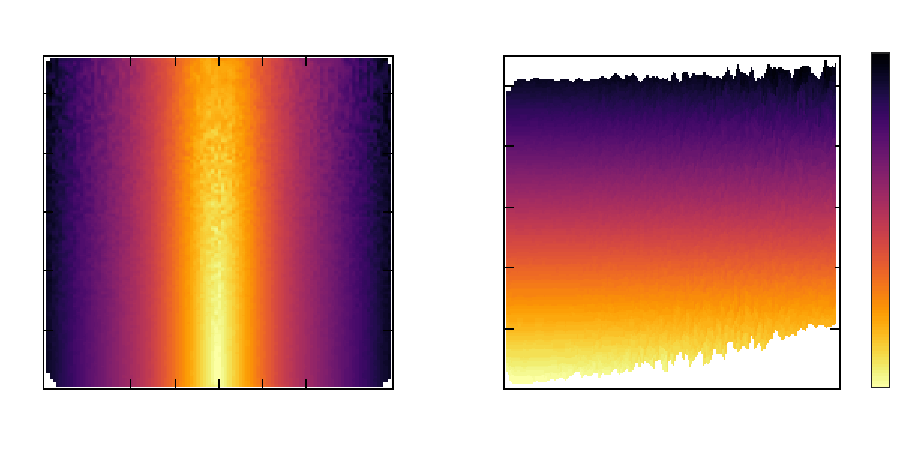
\includegraphics{./figures/parts/02/chapters/04/sections/04/caer_x2}}%
    \gplfronttext
  \end{picture}%
\endgroup

  \end{figure}



\note{\footnotesize

Για να λύσουμε αυτό το πρόβλημα σε γενικές συνθήκες, όπου η εκτίμηση θέσης δεν
είναι ίση με την πραγματική θέση, εφηύραμε τη μετρική CAER, τις οποίας προφίλ
βλέπουμε σε αυτή τη διαφάνεια, η οποία για δεδομένο σφάλμα θέσης εμφανίζει
χαμηλότερες τιμές για χαμηλότερα σφάλματα προσανατολισμού και για δεδομένο
σφάλμα προσανατολισμού χαμηλότερες τιμές για χαμηλότερα σφάλματα θέσης.

}

\end{frame}
